\documentclass[preprint,12pt,authoryear]{elsarticle}
%\documentclass[final,1p,times,twocolumn,authoryear]{elsarticle}
\usepackage{lineno,hyperref}
\modulolinenumbers[5]

\journal{Geoderma}

%%%%%%%%%%%%%%%%%%%%%%%
%% Elsevier bibliography styles
%%%%%%%%%%%%%%%%%%%%%%%
%% To change the style, put a % in front of the second line of the current style and
%% remove the % from the second line of the style you would like to use.
%%%%%%%%%%%%%%%%%%%%%%%

%% Numbered
%\bibliographystyle{model1-num-names}

%% Numbered without titles
%\bibliographystyle{model1a-num-names}

%% Harvard
\bibliographystyle{model2-names.bst}\biboptions{authoryear}

%% Vancouver numbered
%\usepackage{numcompress}\bibliographystyle{model3-num-names}

%% Vancouver name/year
%\usepackage{numcompress}\bibliographystyle{model4-names}\biboptions{authoryear}

%% APA style
%\bibliographystyle{model5-names}\biboptions{authoryear}

%% AMA style
%\usepackage{numcompress}\bibliographystyle{model6-num-names}

%% `Elsevier LaTeX' style
%\bibliographystyle{elsarticle-harv}
%%%%%%%%%%%%%%%%%%%%%%%

\begin{document}

\begin{frontmatter}

\title{Topographic control on soil function evaluation -  a case study from South Tyrol}


%% Group authors per affiliation:

\author[mymainadress]{Fabian E. Gruber\corref{mycorrespondingauthor}}
\cortext[mycorrespondingauthor]{Corresponding author}
\ead{Fabian.Gruber@uibk.ac.at}
\author[mymainadress]{Jasmin Baruck}
\author[secondadress]{Volkmar Mair}
\author[mymainadress]{Clemens Geitner}



\address[mymainadress]{Institute of Geography, University of Innsbruck, Innrain 52f, 6020 Innsbruck, Austria}
\address[secondadress]{ Amt f\"ur Geologie und Baustoffpr\"ufung, Eggentaler Stra{\ss}e 48, 39053 Kardaun, Autonomous Province Bolzano -- South Tyrol, Italy}
\begin{abstract}

\end{abstract}

\begin{keyword}
soil function evaluation, Alpine environment
\end{keyword}

\end{frontmatter}

\linenumbers

\section{Introduction}
Information on soil, a, at least from a human time perspective, non-renewable ressource, is of increasing importance given erosion, soil degradation and soil sealing. It is necessary to know where and where not certain practises are applicable and to adjust land-use planning appropriately. Accordingly, soil function evaluation is an invaluable tool for the future.\newline

\cite{Haslmayr2016} and further literature
\newline

In this study, we present the soil evaluation tool \emph{Soil Evaluation for Planning Procedures (SEPP)} and investigate topographic and parent material control of the different soil functions by applying a cross-validated machine learning approach based on availible soil pit information in the Oltradige/\"{U}beretsch region of the Autonomous Province Bolzano - South Tyrol.
\section{Data and methods}

\subsection{Study area and soil data}

\subsection{SEPP - Soil Evaluation for Planning Procedures}
The software SEPP currently computes a soil function evaluation based on soil pit descriptions. It requires that the pit descriptions are performed following the Austrian Soil classification  \citep{Nestroy2000,Nestroy2011} and related mapping manuals. The minimum  soil profile site characteristics are local slope, thickness of organic horizons, soil depth, groundwater table, soil parent material, soil type, humus form, altitudinal zone, moisture level, land use ... For each horizon, the minimum characteristics necessary for computing the soil function are the master horizon designation, depth, pH value, proportion of the dominant soil structure type and class membership with regard to carbonate content, soil texture, organic content, abundance of rock fragments, bulk density, soil structure. These class attributes can be substituted by exact values if available. The soil functions, for which 15 different potentials are computed, are  \emph{habitat for living organisms} (specifically the potential as habitat for drought-tolerant species, moisture tolerant species, soil organisms and crops),  \emph{infiltration and drainage regulation} (minimum, average and heavy precipitation retention capacity as well as groundwater reformation rate), \emph{natural soil fertility} as well as \emph{filter and buffer for pollutants} (heavy metal, organic, acidifying and water-soluble). The result is a grade between 1 and 5 for each soil function potential, with 1 signifying a high potential and 5 a low one.

\paragraph{Potential as a habitat for drought-tolerant species} 
Both this potential and the following potential as a habitat for moisture-tolerant species are performed based on modifications of the approaches decribed by \cite{BAYGLA2003} and \cite{Lehmann2008}.
The evaluation of a soil's potential  as a habitat for drought-tolerant species is based on the parameters land use, soil type and available field capacity. While the first two parameters are applied to distinguish especially suited (ruderal locations and corresponding soil types) or unsuited (mire deposits and soil types commonly found on these) sites, the latter is used to grade those soil profile sites showing the remaining landuse and soil type combinations. 
\paragraph{Potential as a habitat for moisture-tolerant species}
This potential is evaluated similarly to the the one for drought-tolerant species, in that specific soil types, e.g. Gleysols, are attributed specific grades. In addition, the depth of the groundwater table is used to distinguish sites with high potential, and the available field capacity is used to differentiate even further.
\paragraph{Habitat for soil organisms}

\paragraph{Habitat for crops}

\paragraph{Average and minimum precipitation retention capacity}

\paragraph{Retention capacity for heavy precipitation events}
 
 
\paragraph{groundwater reformation rate}


\paragraph{Potential for providing nutrients for plants}

\paragraph{Potential as a CO2 sink}

\paragraph{Potential for retention of heavy metals}

\paragraph{Potential for transforming organic contaminants}

\paragraph{Potential as filter and buffer for organic contaminants}

\paragraph{Potential for retention of water-soluble contaminants}

\paragraph{Potential as buffer for acidic contaminants}


\section{Results}
The soil function grades for each of the 15 potentials was calculated for each of the 108 soil profile pits in the study area with the SEPP app. Figure \ref{fig:SFdistro} shows the distribution of these grades.
 \begin{figure}[ht!]
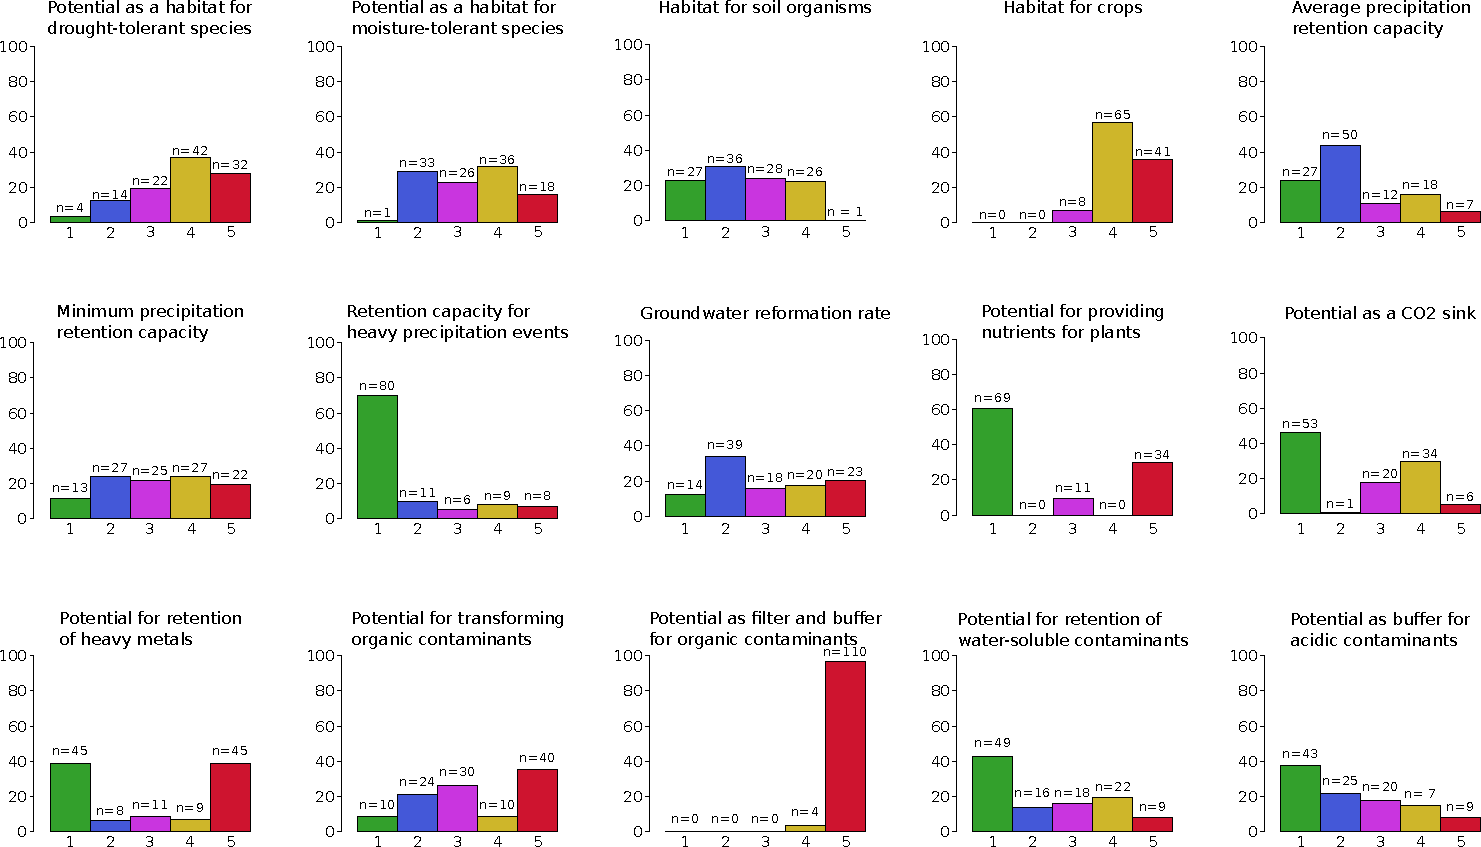
\includegraphics[width=\textwidth,angle=0]{soilfunctiondistro.pdf}
\caption{Barplots representing the distribution of the soil function grades for the various analysed potentials. }
\label{fig:SFdistro}
\end{figure}
A first evaluation of the feature selection procedure shows that mostly 2 parameters are sufficient, that is that there is no increase in cross-validated prediction accuracy  by adding more predictors, and most of the time these a combination of a landform classification and a roughness or also local terrain parameter.
\subsection{Potential as a habitat for drought-tolerant species}
Figure~\ref{fig:SFdistro} shows that of the 108 soil profile sites in the study area, 38 fall into class 4 (35\%) and 32 into class 5 regarding the potential as a habitat for drought-tolerant species. The intermediate class 3 contains 21 soil profiles whereas the high potential classes 1 and 2 are attribute to only 4 and 13 sites, respectively. 
As the predictor set does not contain landuse nor soil type, the SVM classification essentially attempts to model the different classes of available field capacity. In the majority of the feature selection runs a landform map based on a flatness threshold between 3 and 5$^{\circ}$,a spatial resolution of 10~m and a search radius of 100~m was chosen as the first predictive feature. The landform flat is dominant amongst the profile sites with a graded potential of 5, which is accordingly connected to minimal curvature values around 0. The landform slope is  most common for profiles with a potential  of 4, whereas spurs and hollow can present profile locations with a  potential score of 2 and, as expected, have increasingly negative minimum curvature values. A support vector classifier using these two predictor variables results in a cross-validated prediction accuracy of 47\%, where the most common error is that  a large number of sites are mistakenly classified as having grade 4. Nevertheless, the general implications of the feature selection are plausible, as flat areas  can  be expected to have higher field capacity values than sloping regions with negative curvature values.
\subsection{Potential as a habitat for moisture-tolerant species}
\section{Conclusion}
 

\section*{Acknowledgements} This research was performed within the project 'Terrain Classification of ALS Data to support Digital Soil Mapping', funded by the Autonomous Province Bolzano -- South Tyrol (15/40.3).

\section*{References}
\bibliography{P3.bib}u

\end{document}